\chapter{Spiking Associative Memory Architecture and Testing}
\label{chp:spinam}

\marginnote{The spiking implementation of the Willshaw associative memory is no longer truly \enquote{binary} (regarding weights and timings). Therefore the name ``\BiNAM'' might be a little misleading when referring to spiking neural networks; however, the same name is used in this thesis for the sake of consistency.}
The previous chapter introduced the Willshaw associative memory model (\BiNAM) and the notion of spiking neural networks. In this chapter we merge those two concepts: \cref{sec:neural_network_topology} describes the transition of the \BiNAM architecture from a firing-rate coded to a spiking neural network. Furthermore, to account for the spiking network time dynamics, we specify the general testing procedure, how input and output data are encoded as a sequence of spikes, and how noise in the input data is parametrised in a spiking environment. \cref{sec:memory_evaluation_measures} introduces multiple measures for the quantification of the network performance, while \cref{sec:data_generation} focuses on the generation of datasets that can be used for network evaluation.

\section{Neural network topology and data encoding}
\label{sec:neural_network_topology}

\begin{figure}
	\centering
	\subbottom[Single neuron]{
		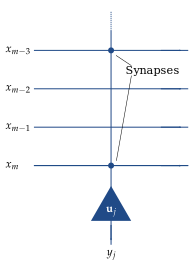
\includegraphics{media/chp3/spinam_topology_a.pdf}
		\label{fig:spinam_topology_a}
	}
	\subbottom[Population of $\populationSize = 2$]{
		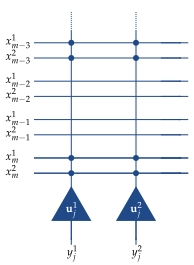
\includegraphics{media/chp3/spinam_topology_b.pdf}
		\label{fig:spinam_topology_b}
	}
	\caption[Comparison between a single neuron BiNAM implementation and its population counterpart]{Two possible implementations of a $j$-th \BiNAM column as spiking neural network: in (a) the network is implemented as a one-to-one translation of the firing-rate neural network topology. In (b) each neuron is replaced by a population of \populationSize neurons ($\populationSize = 2$ in this example); memory input and output components are represented by \populationSize independent signals, $y^1_j, \ldots, y^{\populationSize}_j$.}
	\label{fig:spinam_topology}
\end{figure}

The most trivial way of implementing the Willshaw associative memory model as spiking neural network is to directly employ the firing-rate network topology introduced in \cref{sec:binam_neural_network}: if an entry in the trained storage matrix \((\memMat)_{ij}\) is set to \enquote{one}, a synaptic connection between the neuron $j$ in the output layer and input $i$ in the input layer is established. This basic topology is sketched in \cref{fig:spinam_topology_a}. Another possible topology is shown in \cref{fig:spinam_topology_b}: instead of single neurons, a population of neurons represents each output component, with input and output being transmitted via connection bundles. This topology is presented in detail in \cref{sec:neuron_populations}.

Difficulties in building a spiking neural network arise from the time dynamics: we need to think about how input and output data are represented as a sequence of spikes in the time domain. We consider this problem in more detail in \cref{sec:input_output_time_window,sec:input_data_parametrisation}.

Furthermore, synapse weights are no longer dimensionless scalars which can be trivially mapped to the ones and zeros in \memMat. Instead, each synapse possesses a conductivity measured in siemens. While zeros in \memMat can be mapped to a synapse with zero conductivity (corresponding to no synapse at all), the conductivity $w$ representing a \enquote{one} in \memMat needs to be carefully selected.

\marginnote{Even if we had to implement a \BiNAM as a firing-rate neural network with fixed non-linearity, the threshold could be easily implemented with a sub-network trained for this task via back-propagation. Such a simple training of spiking neural networks is not possible.}
Another problem concerns the threshold in the \BiNAM recall rule from \cref{eqn:binam_recall_rule}: whereas the McCulloch-Pitts neuron model provided a perfect threshold function, single neurons in a spiking neural network do not offer such a well-behaved transfer function. The transfer function is specified as dynamical system which can only be affected by neuron parameter adaptation. This selection of neuron parameters is non-trivial.

In \cref{sec:required_neuron_behaviour}, we discuss the neuron behaviour required for a functioning \BiNAM, given the data representation and the general network topology from the previous sections. We could then try to tune the neuron parameters and synapse weight \(w\) with respect to these rules. This endeavour is the topic of the next chapter \ref{chp:neuron_evaluation}.

\subsection{Input-/output spike sequences}
\label{sec:input_output_time_window}

\begin{figure}
	\centering
	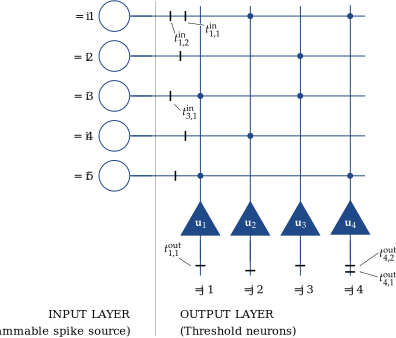
\includegraphics{media/chp3/spinam_nomenclature.pdf}
	\caption[Spiking BiNAM implementation and spike train nomenclature]{Test environment for the spiking implementation of a $5 \times 4$ \BiNAM. The bold marks represent input/output spikes with examples of the spike train nomenclature in \cref{eqn:spike_train_nomenclature}.}
	\label{fig:spinam_nomenclature}
\end{figure}

\begin{figure}
	\centering
	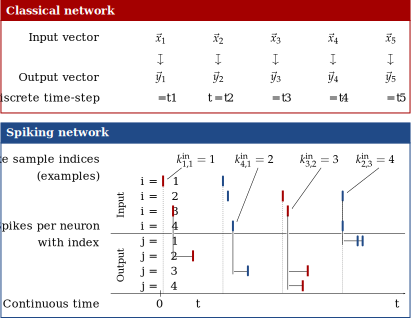
\includegraphics{media/chp3/classical_spiking_comparison.pdf}
	\caption[Comparison between a classical and spiking neural network]{Conceptual comparison between the operation of a classical and spiking neural network: the classical neural network maps between discrete input and output vectors $\vIn_k \mapsto \vOut_k$. Such a mapping has to be artificially created on the input/output of a spiking network by assigning output spikes to the closest past input spike. Dotted vertical lines indicate the first spike belonging to a new sample.}
	\label{fig:classical_spiking_comparison}
\end{figure}

Classical feed-forward firing-rate coded neural networks do not possess time-dynamics: they merely describe a mathematical function $f$ which maps vectorial input $\vIn_k$ onto output $\vOut_k$. The network does not possess any hidden state that may be influenced by previous computations, that is, there are no side-effects. Individual operations -- for example a recall in an associative memory -- are strictly separated from each other. When dealing with time-series of data, an evaluation of $f$ can usually be executed within a single simulation time step.

\marginnote{Of course, separation between individual samples could be forced by repeatedly resetting the simulation. Yet, this may neither be practical (the network state may be important), nor possible (neuromorphic hardware).}
Spiking neural networks do not share these properties: there exists no direct mapping between input and output; both are represented by a stream of continuous spike times, with each spike influencing the state of the involved neurons over time. For closed-loop operation this asynchronicity is one of the defining properties of a spiking neural network. For the sample based performance evaluation of our memory, we need to group input and output spikes that belong to the same sample $(\vIn_k, \vOut_k)$. As network simulations and especially neuromorphic hardware systems do not (or at least not consistently across platforms) allow to dynamically inject spikes during runtime, the entire input spike stream has to be assembled ahead of time and the network output has to be matched in a post-processing step.

To describe our solution to this problem, we first need to specify the spiking \BiNAM test environment (\cref{fig:spinam_nomenclature}): an input layer, a group of \dimIn programmable spike sources, emulates external input to the network. Each source represents a single component $i$ in \(\vIn_k\) and produces a pre-programmed spike train \tInI, which can be described as an ordered sequence of spike times \(t^{\mathrm{in}}_{i,\ell}\)
\begin{align}
	t^{\mathrm{in}}_i &= (
		t^{\mathrm{in}}_{i, 1},
		t^{\mathrm{in}}_{i, 2},
		\ldots) \quad
		    \text{ with } \quad t^{\mathrm{in}}_{i, \ell} \leq t^{\mathrm{in}}_{i, \ell'} \Leftrightarrow \ell \leq \ell' \,.
	\label{eqn:spike_train_nomenclature}
\end{align}

During test execution output spikes \tOutJ are recorded from the output layer, which consists of \dimOut neurons performing the actual thresholding operation. Analogously to the input spike times, \(t^{\mathrm{out}}_{j,\ell}\) denotes the $\ell$-th spike for the $j$-th output component \(\vOut_k\).

In order to assemble \tInI, input samples $\vIn_k$ are converted into their spike time representation (discussed in \cref{sec:input_data_parametrisation}). Let $k^{\mathrm{in}}_{i, \ell}$ denote the sample index each spike $t^{\mathrm{in}}_{i, \ell}$ belongs to. As depicted in \cref{fig:classical_spiking_comparison}, a simple approach for assigning output spikes \(t^{\mathrm{out}}_{j,\ell}\) to the sample $k$ they are most likely associated to, is by selecting $k^{\mathrm{out}}_{j, \ell}$ as the sample index of the latest input spike issued before \(t^{\mathrm{out}}_{j,\ell}\)
\begin{align}
	k^{\mathrm{out}}_{j, \ell} &= k^{\mathrm{in}}_{i, \ell'} \quad \text{with} \quad i, \ell' = \argmin_{i, \ell'}\{t^{\mathrm{out}}_{j,\ell} - t^{\mathrm{in}}_{i,\ell'} \mid t^{\mathrm{out}}_{j,\ell} - t^{\mathrm{in}}_{i,\ell'} > 0 \} \,.
	\label{eqn:spike_train_matching}
\end{align}
In case the network utilises the already mentioned \enquote{neuron population}-topology from \cref{sec:neuron_populations}, there may be multiple neurons for a single input/output component. For sake of simplicity regarding the above equations, we assume that spikes from multiple neurons for the same component $j$ are fused into a single, virtual spike train.

\begin{figure}
	\centering
	\vspace*{0.575cm}
	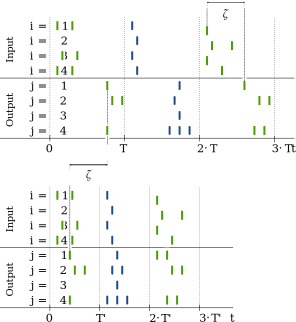
\includegraphics{media/chp3/spike_train_shift.pdf}\\
	\vspace*{0.575cm}
	\caption[Example of input sample pipelining]{Example of input sample pipelining: virtually shifting the output spike times back by $\zeta$ allows higher input sample rate $T'$ while preserving the spike-sample matching (colour coded). Note how the higher sample rate affects the output.}
	\label{fig:spike_train_shift}
\end{figure}
Propagation of a signal through the network is usually not instantaneous. Thus, it can happen that an output spike is mapped to an input spike that already belongs to a later sample. If the minimum delay $\zeta$ between the first input and output spike of a sample is known, the output spike train can be virtually shifted back by $\zeta$ for the calculation of $k^{\mathrm{out}}_{j, \ell}$ according to \cref{eqn:spike_train_matching}
\begin{align}
	i, \ell' = \argmin_{i, \ell'}\{t^{\mathrm{out}}_{j,\ell} - \zeta - t^{\mathrm{in}}_{i,\ell'} \mid t^{\mathrm{out}}_{j,\ell} - \zeta - t^{\mathrm{in}}_{i,\ell'} \geq 0 \} \,.
\end{align}
As shown in \cref{fig:spike_train_shift}, this potentially allows to pack input samples tighter without risking misclassification due to output spikes already being matched with the next sample. The technique can be used to implement pipelining of the memory recall operations. Note however, that due to the statefulness of the network, a higher input sample rate will affect the output.

\subsection{Data encoding and input noise parametrisation}
\label{sec:input_data_parametrisation}

We now need to decide on how to encode a single one-bit as a time sequence of spikes. In case the memory receives input from other networks -- or artificial test data -- which follows this 
specification, we expect our network to respond with another valid output spike pattern in this encoding.
A straight-forward approach is to represent each one-bit in $(\vIn_k$, $\vOut_k)$ as a single spike. So in order to recall a vector for input $\vIn_k$ from the memory, we send a spike to all inputs $i$ with $(\vIn_k)_i = 1$ at a certain time $t = \timeWindow \cdot k$, where the constant \timeWindow is the time between two input samples. The output component $(\vOut_k)_j$ is set to one, if an output spike with assigned sample index \(k^{\mathrm{out}}_{j, \ell} = k\) exists.

We expand this data generation scheme in two ways: by representing ones with potentially more than a single spike, resulting in \emph{bursts}, and by modelling time noise, \emph{jitter}, in the input.

\paragraph{Bursts}
Neurons in the cortex often operate in a \emph{phasic bursting} mode in which action potentials occur in groups of multiple spikes (\cref{fig:isi_decay}), henceforth called \emph{bursts} \cite{connors1990intrinsic}. From a theoretical point of view signalling events using bursts has at least two advantages: they increase the robustness in case of noise -- for example if a single spike out of multiple is lost (as it might happen in both biological and neuromorphic hardware systems), the information about the corresponding event is not irrecoverably destroyed, and if false-positive single spikes are received by a neuron, these can be filtered out \cite{lisman1997bursts}. Secondly, bursts allow to encode analogue values, either by variation of the spike count or the spike frequency within the burst.

To interface with \enquote{bursting} networks our associative memory implementation should support arbitrary integral burst sizes \burstSizeIn and \(\burstSizeOut \geq 1\) chosen at design time. The network has to accept bursts of size \burstSizeIn at the input, but it must also produce \burstSizeOut spikes for each one-bit in the output.

\marginfig{Sketch of a burst with increasing interspike interval}{
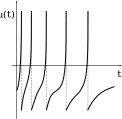
\includegraphics{media/chp3/isi_decay.pdf}
}{Sketch of a neuron membrane potential over time showing spikes from a burst with decaying interspike interval $\isi$.}{\label{fig:isi_decay}}
When generating artificial bursts as test input, we parametrise these with an equidistant \ISI \(\isi\). Note that this is only a coarse model of actual data that might be encountered in a large network, where the interspike interval may be inconsistent: for example in the \AdEx model, the interspike interval is likely to increase over time (\cref{sec:adex} and \cref{fig:isi_decay}). For small \burstSizeIn this effect should be relatively subtle and selecting a constant \isi as the average interspike interval is a reasonable approximation.

On the output side, bursts imply fractional output values whenever a number of spikes that differs from the expected burst size \burstSizeOut is generated. We redefine the value of the output component \((\vOut_k)_j\) as the quotient of the number of actual number of spikes encountered in the output time window, divided by the expected burst size \burstSizeOut
\begin{align}
	(\vOut_k)_j = \frac{| \{k^{\mathrm{out}}_{j, \ell} = k\} |}{\burstSizeOut}
	\label{eqn:spiking_output_values} \,.
\end{align}
To cope with arbitrary \enquote{fractional bit values} in the theoretical \BiNAM storage capacity measure, we introduce an adapted version of the corresponding storage capacity equation (\ref{eqn:binam_entropy_false_negatives}) in \cref{sec:eval_storage_capacity}.

\paragraph{False negative and positive input spikes}
In \cref{sec:binam_failure_modes}, we discussed missing and additional one-bits in the input vectors, where the corresponding events were modelled with probabilities \pFn and \pFp. The representation of one-bits as a series of $\burstSizeIn$ spikes allows to insert and remove individual spikes instead of bits. Thus \pFn is used to describe the probability of skipping a single spike from a burst representing a \enquote{one}, while \pFp describes the probability to issue a single spike from a virtual burst when encoding a \enquote{zero}.

For large burst sizes \burstSizeIn the probability of an entire input burst being removed or added is relatively small (\pFn and \pFp to the power of \burstSizeIn). This is intentional, as the effects of entire bursts being removed and added can be well studied within the theoretical \BiNAM framework (\cref{sec:binam_failure_modes}). For the spiking implementation we want to focus on noise concerning individual spikes instead.

\paragraph{Jitter}
Due to the involved dynamic systems, it is implausible for spiking neural networks to generate perfect timings. In order to emulate these imperfections, we add small time offsets, \emph{jitter}, to the spikes.
\marginnote{Data show that cortical neurons can reproduce spike patters with millisecond precision under laboratory conditions \cite{mainen1995reliability}.}
In our model we sample a random offset from a Gaussian distribution with standard deviation \jitter for each spike time $t^{\mathrm{in}}_{i, \ell}$. Additionally, we shift the entire burst by \jitterMeanOffs in order to model synaptic or spatial delays. Again, \jitterMeanOffs is sampled from a Gaussian distribution with standard deviation \jitterOffs.

\begin{figure}
	\centering
	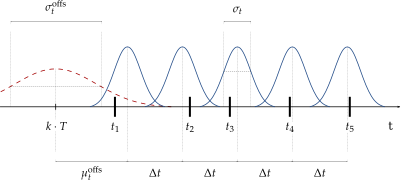
\includegraphics{media/chp3/burst_example.pdf}
	\caption[Parametrisation of an example input spike burst with jitter]{Parametrisation of an example input spike burst of size $\burstSizeIn = 5$ with jitter as described in \cref{eqn:input_spike_burst}. Bold marks correspond to the generated spike times $t_1, \ldots, t_5$. The bell-shaped functions visualise the Gaussian distributions from which the time offset \jitterMeanOffs (dashed) and the individual spike times $t_i$ (blue) are sampled.}
	\label{fig:burst_example}
\end{figure}
\marginnote{As time offsets are drawn from a Gaussian distribution, it might hold $t_{\ell - 1} \geq t_{\ell}$. To allow for computationally efficient processing, a generated sequence of spike times should be sorted in a software implementation.}
An input burst for the $k$-th sample can thus be described as a sequence of \burstSizeIn random variables \((t_1, \ldots, t_{\burstSizeIn})\)
\begin{align}
	t_\ell &\sim \mathcal{N}\Big(k \cdot \timeWindow + \jitterMeanOffs + \isi \cdot (\ell - 1), \jitter\Big) \text{ with } \jitterMeanOffs \sim \mathcal{N}(0, \jitterOffs) \,.
	\label{eqn:input_spike_burst}
\end{align}
Note that the offset \jitterMeanOffs is not an independent random variable for each $t_i$. Instead, it is sampled once for all spike times $t_i$ within the burst.

\begin{table}
	\centering
	\small
	\begin{tabular}{r p{10.1cm}}
		\toprule
		\multicolumn{2}{c}{\spacedlowsmallcaps{Network and input/output parametrisation}} \\
		\midrule
		\multicolumn{2}{c}{\slshape Network and data parameters} \\
		\midrule
		\dimIn, \dimOut & Number of input and output components. \\[0.5em]
		\nOnesIn, \nOnesOut & Number of \enquote{ones} in each input/output sample.\\[0.5em]
		\nSamples & Number of input samples.\\[0.5em]
		\populationSize & Number of neurons representing each output component.\\
		\midrule
		\multicolumn{2}{c}{\slshape Output data parameters} \\
		\midrule
		\burstSizeOut & Output burst size: number of spikes produced by a single neuron in an output burst which represents a \enquote{one}. For neuron populations ($\populationSize > 1$), each individual neuron is expected to produce this number of spikes.\\
		\midrule
		\multicolumn{2}{c}{\slshape Input data parameters} \\
		\midrule
		\burstSizeIn & Input burst size: number of spikes sent in an input burst to a single neuron. For populations, each individual neuron receives $\populationSize$ input bursts of this size.\\[0.5em]
		\timeWindow & Average time between input samples.\\[0.5em]
		\isi & Equidistant interspike interval between input spikes in a burst.\\
		\midrule
		\multicolumn{2}{c}{\slshape Input data noise parameters} \\
		\midrule
		\jitter & Standard deviation of the Gaussian distribution the input spikes are selected from.\\[0.5em]
		\jitterOffs & Standard deviation of the random variable from which the spike burst offset is chosen. Models synaptic or spatial signal delays.\\[0.5em]
		\pFn & Probability of skipping a spike (false-negative) in an input burst when generating a \enquote{one}.\\[0.5em]
		\pFp & Probability of adding a superfluous (false-positive) spike from a virtual input burst when generating a \enquote{zero}.\\
		\bottomrule
	\end{tabular}
	\caption[Network and input/output parametrisation]{Summary of network,  input/output and input noise parameters.}
	\label{tbl:input_data_parametrisation}
\end{table}
\begin{algorithm}
	\small
	\begin{shaded}
		\begin{algorithmic}[1]
			\newcommand{\To}{\textbf{to}\xspace}
			\newcommand{\Init}{\State\textbf{init}\xspace}
			\Function{GenerateInput}{$M, \nSamples, \populationSize, \burstSizeIn, \timeWindow, \isi, \jitter, \jitterOffs, \pFn, \pFp$}
				\Init $t^{\mathrm{in}}_{m, k} \gets () \; \forall \; m \in \{1, \ldots, M\}, k \in \{1, \ldots, \populationSize\}$
				\For{$n \gets 1$ \To $\nSamples$} \Comment{Iterate over all samples}
					\For{$m \gets 1$ \To $\dimIn$} \Comment{Iterate over all input components}
						\If{$(\vIn_n)_m = 1$} \Comment{Set spike omission probability $p$}
							\State $p \gets \pFn$
						\Else
							\State $p \gets 1 - \pFp$
						\EndIf
						\For{$k \gets 1$ \To $\populationSize$} \Comment{Iterate over all neurons in the population}
							\State $t^\mathrm{offs} \gets $ \Call{Normal}{$n \cdot \timeWindow$, \jitterOffs} \Comment{Select burst time offset}
							\For{$\ell \gets 1$ \To $\burstSizeIn$} \Comment{Iterate over all spikes}
								\If{\Call{RandomSelect}{$[0, 1)$}$ \geq p$}
									\State $t^{\mathrm{in}}_{m, k} \gets t^{\mathrm{in}}_{m, k} \Arrowvert $ \Call{Normal}{$t^\mathrm{offs} + (\ell - 1) \cdot \isi$, \jitter}
									\State $k^{\mathrm{in}}_{m, k} \gets k^{\mathrm{in}}_{m, k} \Arrowvert n$
								\EndIf
							\EndFor
						\EndFor
					\EndFor
				\EndFor
				\State $k^{\mathrm{in}}_{m, k} \gets$ \Call{SortByKey}{$k^{\mathrm{in}}_{m, k}, t^{\mathrm{in}}_{m, k}$} $\forall m, k$ \Comment{Sort indices by spike times}
				\State $t^{\mathrm{in}}_{m, k} \gets$ \Call{Sort}{$t^{\mathrm{in}}_{m, k}$} $\forall m, k$ \Comment{Sort spike times}
				\State \Return $\tIn, \kIn$
			\EndFunction
		\end{algorithmic}
	\end{shaded}
	\caption[Input burst generation algorithm]{Input spike train generation algorithm. Generates the input spike trains \tIn and indices \kIn for all neurons according to the data parameters in \cref{tbl:input_data_parametrisation}. For a more consistent notation inside the algorithm, the input dimensionality is denoted as $M$ instead of \dimIn.}
	\label{alg:input_data_generation}
\end{algorithm}
A diagram showing the involved variables is given in \cref{fig:burst_example}, along with an overview of all discussed parameters in \cref{tbl:input_data_parametrisation} and an algorithm for the generation of an input spike sequence for a single input bit $(\vIn_k)_i$ in \cref{alg:input_data_generation}.

\subsection{Neuron populations}
\label{sec:neuron_populations}

\marginnote{The Poisson-distribution
	\[P_\lambda(k) = \frac{\lambda^k}{k!} e^{-\lambda}\]
	describes the probability of an event to occur $k$-times in a certain time interval, given its average rate is $\lambda$.}
Findings regarding neural codes in the cortex suggest that neuron spike patterns can be modelled by a Poisson process \cite{softky1993highly}. This implies that single spike times convey little information -- the instantaneous activity of neural circuitry can only be estimated when pooling responses from multiple neurons. It thus seems likely that neural networks are built redundantly, and information is encoded in the correlation of spike patterns originating from a \emph{population} of neurons \cite{shadlen1994noise}.

With respect to our scenario, the following changes to the network topology take these considerations into account: we replace each neuron $u_j$ with a population of \populationSize neurons $u_j^1, \ldots, u_j^{\populationSize}$, in which each fires a small number of \burstSizeOut spikes per one-bit in the output component $(\vOut)_j$. These neurons receive the same input and all output signals $y_j^1, \ldots, y_j^{\populationSize}$ are fed in parallel to the next input. The signals are treated as a single output $y_j$ for evaluation purposes. As the total number of output spikes for an output component is now given as $\populationSize \cdot \burstSizeOut$, a relatively small burst size can be used (possibly $\burstSizeOut = 1$). Analogously to \cref{eqn:spiking_output_values}, the value of the output component $j$ can be calculated as
\begin{align}
	(\vOut_k)_j = \frac{| \{k^{\mathrm{out}}_{j, \ell} = k\} |}{\populationSize \cdot \burstSizeOut} \,.
	\label{eqn:spiking_output_values_population}
\end{align}

Besides biological plausibility this architecture has two other potential advantages: tuning the neuron parameters in such a way that they produce a small number of spikes might turn out to be easier to accomplish than selecting neuron parameters which cause the neuron to reliably produce an exact large number of output spikes. Furthermore, the redundancy introduced by the neuron populations allows single neurons to fail without severely impacting the network performance.

On the downside, the number of required neurons scales linearly with \populationSize, the number of required synapses scales quadratically with \populationSize, inevitably increasing both size and energy consumption of the network. An example of the topology for $\populationSize = 2$ is sketched in \vref{fig:spinam_topology_b}.

\subsection{Required neuron behaviour}
\label{sec:required_neuron_behaviour}

We have discussed two possible \BiNAM spiking neural network topologies. We now need to specify the neuron behaviour required for the operation of the network. Basically, there are two conditions each neuron in the network must fulfil: the \emph{threshold condition} and the \emph{reset condition}.

\paragraph{Threshold condition}
As specified in the \BiNAM recall rule in \cref{eqn:binam_recall_rule}, the neuron needs to fulfil a thresholding behaviour: let $n_{\mathrm{in}}$ denote the number of input spikes within an input time frame of approximately $\isi \cdot \burstSizeIn$. The number of output spikes the neuron should produce in response to this input is then given as
\begin{align}
	n_{\mathrm{out}}(n_{\mathrm{in}}) &= \begin{cases}
							\burstSizeOut
								& \text{if } n_{\mathrm{in}} \geq \threshOne = \nOnesIn \cdot \burstSizeIn \cdot \populationSize \\
							0
								& \text{if } n_{\mathrm{in}} \leq \threshZero = (\nOnesIn - 1) \cdot \burstSizeIn \cdot \populationSize
	                    \end{cases} \;\;\;\;.
	\label{eqn:threshold_condition}
\end{align}

For input spike counts in the interval $(\threshZero, \threshOne)$, the neuron behaviour is deliberately left undefined, as these values should not occur under perfect conditions and a sharp threshold such as $\threshZero = \threshOne - 1$ would be very demanding to realise.

It should also be stressed, that the neuron parameters for the realisation of the threshold behaviour can only be chosen for a constant time frame $\isi \cdot \burstSizeIn$. At some point, if input spikes arrive in a shorter or longer period of time, more or fewer output spikes will be certainly generated due to the fixed neuron time dynamics. However, we can try to maximise the tolerance to deviations from $\isi \cdot \burstSizeIn$ until a violation of the threshold condition in \cref{eqn:threshold_condition} occurs.

\paragraph{Reset condition}
% \marginfig{Sketch of the reset condition}{TODO}{Sketch of the reset condition. Time windows of length \timeWindow are reserved for a single sample. At the end of each window the neuron should be close to its initial state to avoid interference between samples.}{\label{fig:reset_condition_sketch}}
This condition is closely linked to the way in which we test the network and match output spikes to the input events (\cref{sec:input_output_time_window}): a new sample $k$ with input vector $\vIn_k$ is presented to the network in a fixed interval determined by \timeWindow. All output spikes are interpreted as a response to the sample $k$ to which the last input spike belonged. Correspondingly, the neuron dynamics must ensure that the neuron (a) does not fire any additional output spikes as a response to an input that is longer than \timeWindow ago and (b) is guaranteed to approximately reach its initial condition after a period \timeWindow has passed -- otherwise input samples would influence later tests in an unwanted and uncontrolled way.

\section{Memory evaluation measures}
\label{sec:memory_evaluation_measures}

\marginnote{Note that the presented measures are potentially contradict each other: for example, a network with low energy consumption may exhibit a high latency and small robustness.}
The previous section described the network topology, overall test methodology and two abstract conditions the individual neurons need to fulfil. In this section we discuss various measures for the evaluation of the overall performance of the spiking associative memory implementation: storage capacity, robustness in case of noise, latency and energy consumption.

\subsection{Storage capacity}
\label{sec:eval_storage_capacity}

For a classical \BiNAM the storage capacity evaluation measure has been defined in \vref{eqn:binam_entropy_false_negatives} as entropy of the output samples, minus the entropy of false positives and negatives for each sample $k$. As the binomial coefficient used in the formula classically describes a combinatorial process, it is only defined for integral false positive and negative counts \nFPk and \nFNk. However, in the spiking neural network implementation, those values are derived from fractional bit values \((\vOutKAct)_j\) and are neither integral nor limited to the range expected by the storage capacity formula. The pragmatic solution would be to round the bit values to zero and one. Yet this approach would discard useful information about slight performance degradations.

We thus need to define how to adapt the entropy equation for non-integral values and how to map fractional bit values onto range-limited false positive and negative counts.

\marginnote{An approximation of $\ln(\Gamma(x))$ is provided by most programming environments as a single, numerically stable function.}
The first requirement can be achieved by replacing the faculty operations hidden inside the binomial coefficients with their complex-valued generalisation, the gamma function $\Gamma(x + 1) = x!$. The real-valued generalisation of the binomial coefficient is defined as
\begin{align}
	\lb\binom{n}{k}
		&= \lb\left(\frac{n!}{n! \cdot (n - k)!}\right)
		 = \lb\left(\frac{\Gamma(n + 1)}{\Gamma(k + 1) \cdot \Gamma(n - k + 1)}\right) \notag\\
		&= \lb(\Gamma(n + 1)) - \lb(\Gamma(k + 1)) - \lb(\Gamma(n - k + 1)) \,.
\end{align}
\marginnote{Multiplying $n$ and $k$ in the binomial coefficient by \burstSizeOut seems like another solution to eliminate fractional values. This would imply that the fractional values carry additional information. Strictly speaking this is true, but we never use this information. Our sole goal is to preserve early signs of performance improvement or degradation in the storage capacity measure.}
Given the generalised binomial coefficient we can use the original entropy equation (\ref{eqn:binam_entropy_false_negatives}) with fractional error counts. These are calculated by clamping the fractional bit values to one and linearly accumulating the distance between actual output \((\vOutKAct)_j\) and expected output \((\vOut_k)_j\):
\begin{align}
	\nFPk &= \sum_{j : (\vOut_k)_j = 0} \min \{1, (\vOutKAct)_j \}&
	\nFNk &= \sum_{j : (\vOut_k)_j = 1} 1 - \min \{1, (\vOutKAct)_j \}
\end{align}

With these adaptations the storage capacity measure can be used in conjunction with spiking \BiNAM implementations. In case the neurons fulfil the conditions listed in \cref{sec:required_neuron_behaviour}, the storage capacity measure will return the same values as in the theoretical case, which potentially limits the discriminatory power of the measure. As differentiating between various environments is the primary objective of a benchmark, the discriminatory power might be increased by injecting artificial noise into the simulation and thus obtaining information about the robustness of the current parameter set.

\subsection{Robustness in case of noise}
\label{sec:eval_robustness}

When comparing the robustness of two associative memory implementations in case of noise, we can measure the impact of a certain noise parameter $\eta$ on another evaluation measure -- for example the storage capacity -- under variation of $\eta$. In the remaining section we specify which kind of noise can be addressed and how it is parametrised for testing.

\paragraph{Input noise}
Associative memories are usually designed around \emph{additive/subtractive input noise}: given an arbitrary input vector \vIn, the associative memory should still be capable of returning the output $\vOut_k$ for the sample $k$ with $\| \vIn_k - \vIn \|$ minimal. The robustness in case of this kind of noise can be measured by varying the input noise parameters \pFn and \pFp. Another kind of input noise, \emph{jitter} can be controlled as noise parameters \jitter and \jitterOffs, which control random offsets in the spike timings and randomly model delays in pre-synaptic networks, as well as synaptic or spatial delay. Both noise parameters were described in \cref{sec:input_data_parametrisation}.

\paragraph{Parameter noise}
\marginnote{The iterative digital-to-analogue conversion process used in the NM-PM1 hardware system is an additional source for non-deterministic noise.}
In biological and analogue neuromorphic hardware systems, there are slight deviations in the circuitry which result in two neurons or synaptic connections with supposedly equal configuration to behave differently. In systems based on numeric integration artefacts are introduced by quantisation.

Both deviations can be modelled by artificially adding Gaussian noise to the neuron parameters and synaptic weights: upon network generation we sample a small noise term $\eta$ from a Gaussian distribution with standard deviation $\sigma_{\nParam}$ and add it to the given value for the parameter \nParam. This operation is performed for each neuron and every synaptic connection individually. Care must be taken to clamp the noisy parameter values to their valid range.

\paragraph{State noise}
This term refers to noise present in the state variables (membrane potential, synapse conductivities, adaptation current in \AdEx) of each neuron. In biological systems, spatially close synapses can affect each other although they are not directly connected \cite{barbour1997intersynaptic}. In analogue neuromorphic hardware systems, both thermal noise and crosstalk between neighbouring circuits may superimpose noise onto the neuron state. In software implementations quantisation artefacts can be interpreted as noise superimposed on the state signal (\cf \SQNR \cite{lathi2009modern}). Quantisation artefacts are especially relevant in the many-core neuromorphic hardware system which -- in its current version -- is based on fixed-point numbers with limited resolution.

Artificially injecting this kind of noise into a neural network simulation is not well supported by the software toolchain, so we are unable to analyse the impact of state noise. It should however be kept in mind that this kind of noise exists. The previously mentioned noise models are thus incomplete and cannot be used as the sole explanation of neuromorphic hardware system results.

\subsection{Latency and throughput}
\label{sec:eval_latency}

For conventional digital systems, \emph{latency} describes the time required for the result of an issued operation to be available as output, whereas \emph{throughput} describes the rate new operations can be issued at.

A rather simplistic approach to measuring latency is the following: let $\hat t^{\mathrm{in}}_k$ denote the time of the last input spike and  $\hat t^{\mathrm{out}}_k$ the time of the last output spike associated to a sample $k$ (given that such an output spike exists)
\begin{align}
	\hat t^{\mathrm{in}}_k
		&= \max_{i, \ell} \{t^{\mathrm{in}}_{i, \ell} | k^{\mathrm{in}}_{i, \ell} = k \}\,, &
	\hat t^{\mathrm{out}}_k
		&= \max_{j, \ell} \{t^{\mathrm{out}}_{j, \ell} | k^{\mathrm{out}}_{j, \ell} = k \} \,.
\end{align}
The latency for a single sample $\delta_k$ is now defined as
\begin{align}
    \latency_k = \hat t^{\mathrm{out}}_k - \hat t^{\mathrm{in}}_k \,.
    \label{eqn:latency}
\end{align}

The above definition has two problems. \latency is only well-defined if an output is produced for an input $k$. Furthermore, the actual throughput of the system might be larger than implied by \latency, since the neuron parameters were chosen such that the neuron is ready for the next input sample within a time window \timeWindow. As by definition $\timeWindow > \latency$, the effect of a low latency \latency could be nullified by the delay imposed by \timeWindow until a next sample can be processed.

\marginfig{Sketch of the critical time window measure}{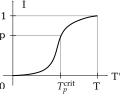
\includegraphics{media/chp3/tcrit.pdf}}{Sketch of the critical time window measure: $T^\mathrm{crit}_p$ is defined as sample interval $\timeWindow'$ at which the relative storage capacity $I$ drops below $p$.}{\label{fig:tcrit}}
A combined measure of latency and throughput is \emph{critical time window} analysis. Instead of presenting samples in the nominal interval \timeWindow, successively smaller $\timeWindow'$ are tested, until the measured storage capacity drops below a relative threshold $p$ of the original storage capacity. The corresponding time window length is called $T^\mathrm{crit}_p$. It corresponds to the maximum frequency at which the memory can be operated without significant impact on its storage capacity (\cref{fig:tcrit}). This approach can of course be combined with the pipelining from \cref{sec:input_output_time_window}.

Certain memory usage patterns might cause interference, which causes the value of $T^\mathrm{crit}_p$ to depend on the input sample order -- however for large sample counts \nSamples this problem should be negligible.

\subsection{Energy}
\label{sec:eval_energy}

Another common evaluation measure for any electronic system is its energy consumption: lower energy consumption implies less heat being dissipated, possibly allowing for higher packing density and overall lower cost of operation. The following considerations should be taken into account for measuring the energy consumption of the associative memory.

For a numerical simulation on a traditional computer architecture, power consumption is mostly influenced by the required simulation time. In analogue neuromorphic hardware however, power consumption is directly related to the neuron state. While modelling the energy consumed by an analogue neuron is out of the scope of this thesis, the required energy $J$ can be roughly modelled as
\begin{align}
	J = \int_{t = 0}^{\infty} (\El - \um(t)) \cdot i(t) \, \mathrm{d}t \,,
	\label{eqn:energy}
\end{align}
where $i(t)$ are the accumulated currents flowing through the neuron membrane.


\section{Data generation}
\label{sec:data_generation}

In the previous sections we have established the foundations for the realisation of a \BiNAM as spiking neural network: we have provided the network topology, a representation of the input data, high-level conditions the spiking neurons need to fulfil and a set of evaluation measures which allow to evaluate the performance of the associative memory. The last missing piece is to describe the actual (non-spiking) data that should be used to test the \BiNAM.

It is important to stress that we do not try to benchmark the \BiNAM itself -- the theoretical limits of this particular associative memory have already been thoroughly studied over the last forty years. Instead, we test a set of particular \BiNAM implementations. Generated data should thus utilise the \BiNAM to the full instead of modelling datasets that may be found in biological systems.

\cref{sec:data_parametrisation} summarises the test data meta parameters. The most obvious candidate for test data -- uncorrelated, random bit vectors -- is discussed in  \cref{sec:binam_random_data_behaviour,sec:random_data_generation}. We then discuss \emph{balanced} datasets, which evenly occupy the \BiNAM and an algorithm which generates such data in \cref{sec:binam_balanced_data,sec:binam_balanced_data_generation}.

\subsection{Dataset parametrisation}
\label{sec:data_parametrisation}

A dataset \(\data = \{(\vIn_k, \vOut_k)\}\) without duplicate input vectors \(\vIn_k\) as defined in \cref{eqn:binam_data} is parametrised by the number of samples \nSamples, the dimensionality of the input and output vectors (\dimIn, \dimOut respectively) and the number of bits set to one in those vectors: \(\|\vIn_k\|_1 = \nOnesIn\) and \(\|\vOut_k\|_1 = \nOnesOut\). The storage capacity formula for hetero-association given in \cref{eqn:binam_entropy_false_negatives} requires the input and output data to be neither inter- nor intracorrelated. Input and output vectors can be represented as a $\nSamples \times \dimIn$ matrix \matIn and a $\nSamples \times \dimOut$ matrix \matOut.

While the perfect test data would produce a minimum number of possible errors while still fulfilling the uncorrelatedness condition, generating such data would require to solve a large binary linear programming problem, which in the general case is NP-complete \cite{karp1972reducibility}. A feasible approach is thus to simply generate random input and output vectors. We discuss the expected behaviour of random data and its generation in the next two sections, followed by a more sophisticated data generation algorithm which ensures uniform usage of the network even for small memory sizes at the cost of violating the uncorrelatedness rule.

\subsection{Expected behaviour in reaction to uncorrelated random data}
\label{sec:binam_random_data_behaviour}

% \marginfig{Example of the false-positive condition}{
% 	\begin{align*}
% 		&~ \hspace{0.95cm}\transpose{\vOut_k} \\
% 		&~ \underline{\begin{matrix} 0 & 1 & 0 & 0 & 1 \end{matrix}} \\
% 		\vIn_k\; \left.\begin{matrix} 0 \\ 1 \\ 0 \\ 1 \end{matrix}\;\right| &~
% 		\underline{\begin{matrix}
% 			0 & 0 & 0 & 0 & 0 \\
% 			{\mathbf{0}} & 1 & {\mathbf{0}} & {\mathbf{0}} & 1 \\
% 			0 & 0 & 0 & 0 & 0 \\
% 			{\mathbf{0}} & 1 & {\mathbf{0}} & {\mathbf{0}} & 1 \\
% 		\end{matrix}} \\
% 		j \;\;\; &~ \begin{matrix} \textit{0} & \textit{1} & \textit{2} & \textit{3} & \textit{4} \end{matrix}
% 	\end{align*}
% }{A false positive arises in component \(j\) of the output for \(\vIn_k\), exactly if all highlighted zeros in column \(j\) of \memMat are set to one.}{\label{fig:binam_false_positive_condition}}
In order to analyse the expected behaviour of random data in the \BiNAM we first need to understand the conditions under which errors occur if non-noisy input data is given. As described in \cref{sec:binam_failure_modes} the only kind of errors in the output of a theoretical \BiNAM with perfect input are false positives. According to \cref{eqn:binam_recall_rule}, for an input \(\vIn_k\) a false positive will arise at position $j$ of the output (for which \((\vOut_k)_j = 0\)) exactly if
% (\cref{fig:binam_false_positive_condition}):
\begin{align}
	(\transpose{\memMat} \cdot \vIn_k)_j = \sum_{i : (\vIn_k)_i = 1} (\memMat)_{ij} \overset{!}= \|\vIn_{k}\|_1 = \nOnesIn \,.
	\label{eqn:binam_false_positive_condition}
\end{align}
In other words: a false positive in output component $j$ for a sample $(\vIn_k, \vOut_k)$ is generated if for each \enquote{one} at position \(i\) in \(\vIn_k\) there exists a sample $k'$ with \((\vOut_{k'})_j = 1\) and \((\vIn_{k'})_i = 1\) \cite{palm1980associative}. The condition of an additional one occurring at position $j$ in the output for \(\vIn_k\) is henceforth abbreviated as \(C(k, j)\). If we neglect that there may be no duplicate input vectors \(\vIn_k\), the expected total number of false positives per sample \(\langle n_{\mathrm{fp}} \rangle\) can be easily calculated.

\marginnote{The probability \(\wp\) is the same for all cells \(i\), \(j\) since the bits are distributed independently and uniformly across the input and output vectors.}
\marginnote{If we wanted to respect the fact that there are no duplicates in the entirety of \(\vIn_k\), we would not be allowed to express \(\probability{((\memMat)_{i, j} = 0)}\) as a product: the individual events are no longer independent. However, the error introduced by this assumption is sufficiently small for large memories \cite{palm1980associative}.}
Let $\wp$ denote the probability of a single cell \(i\), \(j\) in \memMat being set to one after \nSamples samples have been trained
\begin{align}
	\wp &= \probability{((\memMat)_{i, j} = 1)} = 1 - \probability{((\memMat)_{i, j} = 0)} \\
		&= 1 - \prod_{k = 1}^{\nSamples} \probability{((\vIn_k)_i = 0 \vee (\vOut_k)_j = 0)} \\
		&= 1 - \prod_{k = 1}^{\nSamples} \left(1 - \probability{((\vIn_k)_i = 1 \wedge (\vOut_k)_j = 1)} \right) \\
		&= 1 - \prod_{k = 1}^{\nSamples} \left(1 -
			\probability{((\vIn_k)_i = 1)} \cdot \probability{((\vOut_k)_j = 1)}\right) \\
		&= 1 - \left(1 - \frac{\nOnesIn \cdot \nOnesOut}{\dimIn \cdot \dimOut}\right)^{\nSamples} \,.
\end{align}
According to \cref{eqn:binam_false_positive_condition} the probability $\probability{(C(k, j))}$ of a false positive occurring in the $j$-th component of sample $k$ can be described as
\begin{align}
\probability{(C(k, j))} &= \probability{\left((\transpose{\memMat}
			\cdot (\vIn_k))_j = \nOnesIn\right)}
		 = \probability{\left(
			\sum_{i = 1}^{\dimIn} (\memMat)_{i, j} \cdot (\vIn_k)_i = \nOnesIn \right)} \label{eqn:ckj_1}\\
		&= \probability{\left(
			\sum_{i = 1}^{\dimIn} \left(\bigvee\nolimits_{\ell = 1}^{\nSamples} (\vIn_\ell)_i \cdot (\vOut_\ell)_j \right) \cdot (\vIn_k)_i = \nOnesIn \right)} \label{eqn:ckj_2}\,.
\end{align}
Since \((\vOut_k)_j = 0\) (otherwise a one in the $j$-th output component would be a \emph{true} positive), we can add the condition $\ell \neq k$ to the inner \enquote{$\vee$}-operation of \cref{eqn:ckj_2} without changing its value
\begin{align}
\probability{(C(k, j))} &= \probability{\left(
			\sum_{i = 1}^{\dimIn} \left(\bigvee\nolimits_{\ell = 1, \ell \neq k}^{\nSamples} (\vIn_\ell)_i \cdot (\vOut_\ell)_j \right) \cdot (\vIn_k)_i = \nOnesIn \right)} \label{eqn:ckj_3} \,.
\end{align}
Now it is clearly visible that there is no dependence between \(\memMat\) and \(\vIn_k\) in \cref{eqn:ckj_1}. The final $\probability{(C(k, j))}$ is thus given as
\begin{align}
\probability{(C(k, j))} &= \probability{\left(
			\bigwedge\nolimits_{i : (\vIn_k)_i = 1} (\memMat)_{i, j} = 1 \right)}
			= \wp^{\nOnesIn} = \left(1 - \left(1 - \frac{\nOnesIn \cdot \nOnesOut}{\dimIn \cdot \dimOut}\right)^{\nSamples}\right)^{\nOnesIn} \,.
\end{align}
\marginnote{For large \dimIn, \dimOut the error caused by allowing duplicates in \matIn diminishes. A proof is given in appendix B of \cite{palm1980associative}.}
The expected number of false positives \(\langle n_{\mathrm{fp}} \rangle\) per sample \(k\) for uncorrelated, randomly generated input and output vectors is consequently
\begin{align}
\langle n_{\mathrm{fp}} \rangle = (\dimOut - \nOnesOut) \cdot \left(1 - \left(1 - \frac{\nOnesIn \cdot \nOnesOut}{\dimIn \cdot \dimOut}\right)^{\nSamples}\right)^{\nOnesIn} \,.
\label{eqn:expected_err}
\end{align}
\begin{figure}
	\centering
	\includegraphics[trim=0cm 5.5cm 0cm 0cm,clip]{media/chp3/expected_err.pdf}\\
	\includegraphics[trim=1.5cm 0cm 2.5cm 2cm,clip]{media/chp3/expected_err.pdf}
	\includegraphics[trim=1.5cm 0cm 2.5cm 2cm,clip]{media/chp3/expected_info.pdf}
	\caption[Estimated number of false positives]{Estimated number of false positives per sample \(k\) and corresponding information \(I\) for varying memory size \(\dimIn, \dimOut\) and number of bits set \(\nOnesIn, \nOnesOut\).}
	\label{fig:expected_err}
\end{figure}\ignorespaces
\cref{fig:expected_err} shows \( \langle n_{\mathrm{fp}} \rangle \) and the corresponding information estimate for a varying number of samples \nSamples and different combinations of \dimIn, \dimOut, \nOnesIn, \nOnesOut.

\subsection{Random data generation algorithm}
\label{sec:random_data_generation}

Input and output vector matrices \matIn, \matOut are independently generated as data blocks $\matData = \transpose{(\vec b_1, \ldots, \vec b_{\nSamples})}$, where each $\vec b_i$ is an $r$-tuple containing $r_1$ ones and $r_0 = r - r_1$ zeros
\begin{align}
	\vec b_i \in \mathfrak{B}^r_{r_1} = \left\{(b_{1}, \ldots, b_{r}) \,\middle|\, b_j \in \B, \sum\nolimits_{j = 1}^r b_j = r_1 \right\} \,.
\end{align}
According to basic combinatorics the size of \(\mathfrak{B}^r_{r_1}\) is
\begin{align}
	|\mathfrak{B}^r_{r_1}| = \binom{r}{r_1} = \binom{r}{r - r_1} = \binom{r}{r_0} \,.
\end{align}
\marginfig{Example bit vectors and their set representation}{
$(1, 0, 1, 0, 0) \rightarrow \{0, 2\}$ \\[0.25em]
$(0, 0, 1, 0, 1) \rightarrow \{2, 4\}$ \\[0.25em]
$(0, 1, 0, 0, 1) \rightarrow \{1, 5\}$ \\[0.5em]}{Elements of $\mathfrak{B}^5_2$ and their corresponding set representation.}{\label{fig:permutations_compact_example}}
Each vector $\vec b \in \mathfrak{B}^r_{r_1}$ can be uniquely represented as set $\mathfrak{b}$ containing the indices of \enquote{ones} in $\vec b$ (\vref{fig:permutations_compact_example})
\begin{align}
	\mathfrak{b} &= \{i \mid b_i = 1\} & \mathfrak{b} \in \mathfrak{b}^r_{r_1} &= \{\{i_1, \ldots, i_{r_1}\} \mid i_j \in \{1, \ldots, r\}\} \,.
\end{align}
\begin{algorithm}
	\small
	\begin{shaded}
		\begin{algorithmic}[1]
			\newcommand{\To}{\textbf{to}\xspace}
			\newcommand{\Init}{\State\textbf{init}\xspace}
			\Init \(\matData \gets 0 \in \B^{\nSamples \times r}\) \Comment{Result matrix}
			\For{ \(i \gets 1\) \To \nSamples}
				\For{ \(j \gets r - r_1 + 1\) \To \(r\)}
					\State \(\ell \gets \) \Call{RandomSelect}{$\{1, \ldots, j - 1\}$} \Comment{Uniformly select set entry}
					\If{\({\matData}[i,\ell] = 1\)}
						\State \({\matData}[i,j] \gets 1\)
					\Else
						\State \({\matData}[i,\ell] \gets 1\)
					\EndIf
				\EndFor
			\EndFor
		\end{algorithmic}
	\end{shaded}
	\caption[Uncorrelated random data generation]{Algorithm for the generation of a block $\matData$ of \nSamples uncorrelated random vectors of length $r$, containing exactly $r_1$ ones.}
	\label{alg:binam_random_data}
\end{algorithm}\ignorespaces
The set $\mathfrak{b}^r_{r_1}$ is the set of all $r_1$-sized sets over $\{1, \ldots, r\}$, or -- in mathematical terms -- the set of all $r_1$-combinations of $\{1, \ldots, r\}$. As shown in \cref{alg:binam_random_data} a set of $n$ random $r_1$-combinations can be efficiently generated in $\mathcal{O}(n \cdot r_1)$ time \cite{bentley1987programming}.

This algorithm does not ensure the absence of duplicates in the input. While the probability of a duplicate is sufficiently small for large \dimIn, one could expand the algorithm by a hash-table lookup and retry if a vector has already been generated. Yet such a method may not terminate if an exhaustively large dataset is generated. An alternative which is guaranteed to terminate is the algorithm presented in \cref{sec:binam_balanced_data_generation}.

\subsection{Balanced data}
\label{sec:binam_balanced_data}

\begin{figure}
	\centering
	\includegraphics{media/chp3/binam_occupancy_data.pdf}
	\caption[Comparison of the BiNAM matrix occupancy for different data generation methods]{Comparison of the \BiNAM matrix occupancy distribution for different data generation methods: the occupancy measures how many times a \BiNAM matrix cell would be set to one during training. Training was simulated for hetero-association with $100$ samples in a $32 \times 32$ \BiNAM with $\nOnesIn = \nOnesOut = 16$ one-bits for each vector. The box plots visualise the distribution of the occupancy values for $1000$ independent training runs over all matrix cells (the box extends from the lower to the upper quartile, with a line at the median, the whiskers depict the 1.5 interquartile range, crosses outliers).}
	\label{fig:binam_occupancy_data}
\end{figure}

For practical experiments with relatively small networks, uncorrelatedness does not guarantee a uniform occupancy of the storage matrix bits, as the probability for two randomly generated samples to activate the same bits in \memMat increases with smaller memories. This might be a problem when benchmarking neuromorphic hardware systems, where we would like to ensure that at any time during the test run all neurons and synapses get approximately the same workload in order to produce a more stable behaviour.

The introduction of the \emph{balancing} condition -- besides uncorrelatedness and uniqueness of the input vectors -- allows to ensure this. For any $k' \leq \nSamples$ the column sums of a generated data block $\matData$ (which may either refer to the input data \matIn or the output \matOut) must be balanced. Specifically, it must hold
\begin{align}
	\max_j\left\{\sum\nolimits_{k = 1}^{k'} \matData_{kj}\right\} - \min_j\left\{\sum\nolimits_{k = 1}^{k'} \matData_{kj}\right\} \leq 1 \, \forall k' \leq \nSamples \,.
	\label{eqn:balancing_condition}
\end{align}
A potential effect of the balancing is shown in \cref{fig:binam_occupancy_data}: when calculating how many times a cell in the \BiNAM is set to one during training -- which can be computed as  $X^T \cdot Y$ -- the variance in occupancy significantly reduces when balancing is enabled.

An alternative interpretation of the balancing rule is a prolonged creation of false positives, which in return increases the information that can be stored in the \BiNAM: input and output data balancing selects rows and columns in the \BiNAM which have not yet been used as often as others, lowering the probability of the false-positive condition $C(r, j)$. An experiment showing this effect is depicted in \cref{fig:binam_data_information_comparison} -- balanced vectors without duplicates for both input and output data achieves the highest \BiNAM storage capacity.

\marginfig{Example of correlation introduced by data balancing}{
$\vec b_1 = (0, 1, 0, 0, 1, 1)$\\
$\vec b_2 = (1, 0, 1, 1, 0, 0)$\\
$\vec b_3 = (1, 1, 0, 0, 0, 1)$\\
$\vec b_4 = (0, 0, 1, 1, 1, 0)$\\
\vspace{0.25cm}
}{Correlation introduced by data balancing for $r = 6$ and $r_1 = 3$: while the data generation algorithm can randomly select $\vec b_1$ and $\vec b_3$, samples $\vec b_2$ and $\vec b_4$ are predetermined.}{\label{fig:data_balancingelation}}
Unfortunately, these results must be taken with a grain of salt: from a strict mathematical point of view, balancing causes intracorrelation in a dataset $\matData$ (\cref{fig:data_balancingelation}). Therefore the storage capacity formula from \cref{eqn:binam_entropy_false_negatives} cannot be applied. However, we believe that the introduced correlation (similarly to requiring no duplicates in the input) is sufficiently small for any reasonably large number of samples \nSamples. After all, an algorithm generating balanced data could still generate all possible data vectors, though it limits the random selection in each step to those vectors which fulfil the balancing condition in \cref{eqn:balancing_condition}.
\begin{figure}
	\small
	\centering
	\subbottom[Homogeneous data generation method. Both \vIn and \vOut are without duplicates.]{
		\includegraphics[trim=0cm 0.2cm 0cm 0.3cm, clip]{{media/chp3/binam_data_information_16_3_100_1000_no_duplicates.mat}.pdf}
		\label{fig:binam_data_information_comparison_no_duplicates}
	}
	\subbottom[Heterogeneous data -- \vIn is without duplicates, \vOut potentially with duplicates.]{
		\includegraphics[trim=0cm 0.2cm 0cm 0.3cm, clip]{{media/chp3/binam_data_information_16_3_100_1000_input_output.mat}.pdf}
		\label{fig:binam_data_information_comparison_input_output}
	}
	\caption[Random versus balanced data generation]{Random versus balanced data generation. $1000$ trials in which a $16 \times 16$ \BiNAM with $3$ ones in input/output is incrementally trained with \nSamples samples were conducted. Samples are either generated randomly, or randomly with balanced bit allocation. The bold line depicts the median information, the dotted line the trial with maximum information and the dashed line the prediction according to \cref{eqn:expected_err}. The $25/75\%$-quantile and the minimum/maximum over all trials are shaded. (a) shows the experiment for input and output data homogeneously generated with one of the two methods, (b) explores the heterogeneous case.}
	\label{fig:binam_data_information_comparison}
\end{figure}


\subsection{Balanced data generation algorithm}
\label{sec:binam_balanced_data_generation}

\begin{figure}
	\centering
	\subbottom[Root node in the initial state of the algorithm.]{%
		\begin{minipage}[b][4cm][t]{0.4675\textwidth}
			\centering
			\includegraphics{media/chp3/data_generation/out/algorithm_000_cropped.pdf}
		\end{minipage}
	}
	\quad
	\subbottom[Updated tree after the selection of the first \enquote{one} at index three.]{%
		\begin{minipage}[b][4cm][t]{0.4675\textwidth}
			\centering
			\includegraphics{media/chp3/data_generation/out/algorithm_001_cropped.pdf}
		\end{minipage}
	}
	\caption[Balanced data generation algorithm example 1]{Example of the data generation algorithm with $r = 5$ and $r_1 = 3$. The bold frame indicates the currently active node $\aleph$. In (a) none of the bits have been used yet. Indices $1$ or $2$ (hatched) can not be chosen as this would not leave a sufficient number of indices to choose from for the remaining bits. In (b) the index $4$ has been selected: the usage count is incremented, the number of remaining permutations starting with $4$ is decremented in the root node. Only bit indices $2$ and $3$ are viable next child indices for the new node.}
	\label{fig:binam_balanced_data_generation_algo1}
\end{figure}
\marginnote{A \enquote{prefix-tree} or \enquote{Trie} is a standard data-structure in computer-science used for compact storage of a set of sequences. Common prefixes are represented by a single node. Whenever the sequences diverge the Trie branches \cite{knuth1998trie}.}
Subsequently we present a simple and fast algorithm for the generation of \nSamples random and balanced bit vectors without duplicates. As in \cref{alg:binam_random_data}, the method is based on the set representation $\mathfrak{b}_k$ of a bit vector $\vec b_k$, and the one-bit indices are chosen one at a time.

The key idea of the algorithm is to induce an order on the possible $r_1$-combinations by representing them as a sequence of one-indices $(i_1, \ldots, i_{r_1})$ with $i_{j} > i_{j'} \Leftrightarrow j' > j$. These sequences are organised in a prefix-tree -- \emph{Trie} -- of depth $r_1 + 1$: each node represents the index of a single one-bit, every possible path from the root node to a leaf represents a unique combination. This properties allows to track how many not-yet-generated combinations are reachable from a node.

\marginnote{The root node $\aleph^\perp$ can be seen as a virtual node with index $i = r + 1$ at level $\ell = 0$.}
For each Trie node $\aleph$ with index $i$ at level $\ell$ we initially calculate a table containing the number of possible combinations for each child $j < i$ and $\tilde r = r_1 - \ell$ remaining ones
\begin{align}
	\aleph^{\to j} = |\mathfrak{b}^j_{\tilde r}| = \begin{cases}
		\binom{j}{\tilde r} & \text{if } j \geq \tilde r \\
		0 & \text{if } j < \tilde r
	\end{cases} \,.
	\label{eqn:possible_paths}
\end{align}
Whenever a path along a child node $\aleph[j]$ is traversed, the corresponding table entry $\aleph^{\to j}$ is decremented, as a new combination with this path as prefix is being generated. Once $\aleph^{\to j}$ is zero, the corresponding path is ignored in future index selections (\cref{fig:binam_balanced_data_generation_algo1,fig:binam_balanced_data_generation_algo2}).

\begin{figure}[p]
	\centering%
	\includegraphics[trim=0.25cm 0cm 1.4cm 0cm, clip]{media/chp3/balanced_no_bias.pdf}%
	\includegraphics[trim=1.25cm 0cm 0cm 0cm, clip]{media/chp3/balanced_with_bias.pdf}%
	\caption[Linear correlation coefficient with and without index selection bias]{Linear correlation coefficient for two bits $i$, $j$ in 10000 generated bit vectors with a length of $r = 128$ and $r_1 = 3$ ones. The left plot shows the result for data generated with disabled selection bias, the right with enabled selection bias.}
	\label{fig:balanced_bias}
\end{figure}
\begin{algorithm}[p]
	\small
	\begin{shaded}
		\begin{algorithmic}[1]
			\newcommand{\To}{\textbf{to}\xspace}
			\newcommand{\Init}{\State\textbf{init}\xspace}
			\Function{Balancable}{$\vec u, i, \tilde r$}
				\State \(\triangleright\) \textit{Indices which allow balancing of at least $\tilde r - 1$ future ones}
				\State \Return \(\left\{ j \,\middle\vert\, \sum_{j' = 1}^{j} \max\{0, 1 - \vec u[j'] + \min(\vec u)\} \geq \tilde r, j \in \{1, \ldots, i - 1\} \right\}\)
			\EndFunction\vspace{0.25cm}
			\Function{Generate}{$\nSamples, r, r_1$}
				\Init \(\matData \gets 0 \in \B^{\nSamples \times r}\) \Comment{Result matrix}
				\Init \(\vec u \gets 0 \in \N^r\) \Comment{Bit usage count vector}
				\Init \(\aleph^\perp\) \Comment{Initialise root node}
				\For{ \(n \gets 1\) \To \nSamples} \Comment{Iterate over all \nSamples samples}
					\State \(\aleph \gets \aleph^\perp, i \gets r + 1\) \Comment{Current node, start with root}
					\For{ \(\ell \gets 0\) \To \(r_1 - 1\)} \Comment{Trie level $\ell$}
						\State \(\tilde r \gets r_1 - \ell\) \Comment{Number of remaining one-bits $\tilde r$}
						\State \(\mathfrak{s} \gets \{j \mid \aleph^{\to j} > 0 \}\) \Comment{Indices with remaining paths}
						\State \(\mathfrak{s} \gets \mathfrak{s} \cap \{j \mid \vec u[j] = \min \{ \vec u[j'] \mid j' \in \mathfrak{s}\}\}\) \Comment{Balance bit usage}
						\If{\Call{Balancable}{$\vec u, i, \tilde r$} $\, \cap \; \mathfrak{s} \neq \emptyset$}
							\State \(\mathfrak{s} \gets\) \Call{Balancable}{$\vec u, i, \tilde r$} \(\, \cap \; \mathfrak{s} \)
						\EndIf
						\State \(j \gets\) \Call{WeightedRandomSelect}{$\{(j, \aleph^{\to j}) \mid j \in \mathfrak{s} \}$}
						\State \(\matData[n, j] \gets 1\) \Comment{Set output bit}
						\State \(\vec u[j] \gets \vec u[j] + 1\) \Comment{Increment bit usage count}
						\State \(\aleph^{\to j} \gets \aleph^{\to j} - 1\) \Comment{Decrement remaining path count}
						\State \(\aleph \gets \aleph[j], i \gets j\) \Comment{Go to child node $j$}
					\EndFor
				\EndFor
			\EndFunction
		\end{algorithmic}
	\end{shaded}
	\caption[Uncorrelated, random and unique data generation]{Algorithm for the generation of a block $\matData$ of \nSamples unique, uncorrelated random vectors of length $r$, containing exactly $r_1$ ones with balanced bit allocation. Skipping lines 14--17 deactivates bit allocation balancing. \cref{eqn:possible_paths} describes how to initialise $\aleph^{\to j}$ upon first access. See text for description.}
	\label{alg:binam_balanced_data}
\end{algorithm}
For each of the \nSamples vectors, child indices $j$ are randomly selected from the possible child indices, moving the current-node cursor $\aleph$ through the Trie. As soon as the lowest Trie level is reached after $r_1$ choices, the cursor is reset to the root $\aleph^\perp$ and the next vector is generated. An important detail is to bias the index selection by the number of possible paths continuing with $j$, $\aleph^{\to j}$. Failing to add the selection bias results in intracorrelation: if the first chosen bit index $j$ is small, the next indices that can be selected must be smaller than $j$, causing small bit indices to appear in groups. This effect is shown in \cref{fig:balanced_bias}: whereas there is a strong linear intracorrelation between lower (and as a result of balancing also higher) bit indices, the selection bias reduces the linear correlation coefficient between arbitrary bit indices to a small, uniform noise.

\begin{figure}
	\centering
	\subbottom[Child node $j = 2$ is selected and inserted.]{%
		\begin{minipage}[b][7.5cm][t]{0.4675\textwidth}
			\centering
			\includegraphics{media/chp3/data_generation/out/algorithm_002_cropped.pdf}
		\end{minipage}
	}
	\quad
	\subbottom[The first $r_1$-combination $(4, 2, 1)$ has been generated, the cursor is reset to $\aleph^\perp$.]{%
		\begin{minipage}[b][7.5cm][t]{0.4675\textwidth}
			\centering
			\includegraphics{media/chp3/data_generation/out/algorithm_003_cropped.pdf}
		\end{minipage}
		\label{fig:binam_balanced_data_generation_algo2_b}
	}
	\caption[Balanced data generation algorithm example 2]{Continuation of the data generation algorithm example from \cref{fig:binam_balanced_data_generation_algo1}. In (a) child node $2$ has been selected. Consequently, the only possible final node for this combination is $j = 1$. As indicated by the red usage count in (b), the index $4$ cannot be chosen, as there are possible bits which have been used fewer times. The yellow usage count indicates an index with minimal usage count, but whose selection would not allow to balance the bit usage of larger indices. The remaining choice is to select bit index $5$.}
	\label{fig:binam_balanced_data_generation_algo2}
\end{figure}
\begin{figure}
	\centering
	\includegraphics{media/chp3/data_generation/out/algorithm_019_cropped.pdf}
	\caption[Balanced data generation algorithm example 3]{In certain situations the only possible choice introduces temporarily unbalanced vectors -- either index $2, 3$ or $4$ must be chosen at the current node, although their bit usage is not minimal.}
	\label{fig:binam_balanced_data_generation_algo3}
\end{figure}

\marginnote{Note that in \cref{fig:binam_balanced_data_generation_algo2_b} $(0, 0, 1, 1, 1)$ would be a possible next vector, but the algorithm can only generate $(0, 1, 1, 0, 1)$ or $(1, 0, 1, 0, 1)$ due to its greedy balancing strategy. We believe that fixing this issue is not worth the benefits: for reasonably large $r$ the probability for such correlations is small.}
Until now the algorithm generates \nSamples random and unique $r_1$-combinations. It does not fulfil the balancing condition from \cref{eqn:balancing_condition}. Balancing can be achieved by keeping track of the usage count of each bit index in a vector $\vec u \in \N^r$: whenever a bit index $j$ is selected, the corresponding entry $(\vec u)_j$ is incremented by one. We then restrict the set of currently selectable bit indices $\mathfrak{s}$ to those for which the usage count is minimal
\begin{align}
	\mathfrak{s}_{\mathrm{min}} &= \mathfrak{s} \cap \{j \mid (\vec u)_j = \min\{(\vec u)_{j'} \mid j' \in \mathfrak{s}\}\} & \text{where } \mathfrak{s} = \{j \mid \aleph^{\to j} > 0\} \,.
\end{align}
As shown in \cref{fig:binam_balanced_data_generation_algo2_b}, this basic approach has to be refined: it may happen, that a bit index $j$ has minimal usage. However, as we select the largest $j$ in each step, there might be cases in which its selection would prevent a larger bit index to be balanced. We therefore calculate the bit indices $\mathfrak{s}_{\mathrm{bal}}$ which allow the selection of at least $\tilde r = r_1 - \ell$ remaining ones with minimal usage
\begin{align}
	\mathfrak{s}_{\mathrm{bal}} &= \left\{ j \;\middle\vert\; \sum\nolimits_{j' = 1}^{j} \max\{0, 1 - (\vec u)_{j'} + \min(\vec u)\} \geq \tilde r, j \in \{1, \ldots, i - 1\} \right\} \,.
\end{align}
The final selectable indices $\mathfrak{s}_{\mathrm{sel}}$ are then given as
\begin{align}
	\mathfrak{s}_{\mathrm{sel}} &= \begin{cases}
									\mathfrak{s}_{\mathrm{min}} \cap \mathfrak{s}_{\mathrm{bal}} & \text{if } \mathfrak{s}_{\mathrm{min}} \cap \mathfrak{s}_{\mathrm{bal}} \neq \emptyset \\
									\mathfrak{s}_{\mathrm{min}} & \text{otherwise}
	                               \end{cases} \,.
\end{align}
Rationale for the second case is given in \cref{fig:binam_balanced_data_generation_algo3}: in intermediate steps it may be necessary to generate a temporarily unbalanced bit usage.

\cref{alg:binam_balanced_data} shows pseudo-code describing the method in its entirety. With $\mathcal{O}(\nSamples \cdot r_1 \cdot r)$ the runtime of the method linearly depends on \nSamples and $r$, which is worse than the previously presented $\mathcal{O}(\nSamples \cdot r_1)$ algorithm for non-balanced, non-unique samples.

\section{Conclusion}

This chapter outlined the design space of spiking \BiNAM implementations: apart form the actual neuron parameters, the design space consists of the data parameters, the population size and the chosen input and output signal encoding (\cf \cref{tbl:input_data_parametrisation}). Furthermore, we discussed the network testing procedure and possible evaluation measures, as well as different test sample generation schemes, for which we presented efficient algorithms.

Regarding the latter, experiments show that balanced input and output vectors $(\vIn_k, \vOut_k)$ without duplicates produce a more uniform activation of the synapses during experiments and achieve a higher possible storage capacity than randomly selected vectors.

With the material presented in this chapter we could implement a design space exploration pipeline which performs data generation, network construction, actual simulation on either a software integrator or one of the neuromorphic hardware systems, and evaluation according to the proposed measures.

However, such full network simulations are time-consuming and of limited feasibility for parameter optimisation with respect to one of the measures. \cref{chp:neuron_evaluation} will thus approach the problem from a higher abstraction level and introduce estimations which predict the performance of a given neuron parameter set \nParams for the network parameters listed above. We then move to the actual full network experiments on neuromorphic hardware in \cref{chp:experiments}.
